% theroy syntethic images
Synthetic images are computer-generated images that simulate real-world scenes or objects. They are increasingly used in computer vision when collecting real-world data is either difficult, expensive or raises privacy concerns. These images are especially useful for training machine learning models for tasks like object detection and image classification. When generating synthetic data, developers can create datasets that meet specific needs, which is important for industries like healthcare, self-driving cars and near-shore ocean environment, where real-world data may be hard to gather \cite{jimaging8110310, safety}.

\section{Advantages of Synthetic Data for CV Models}

Deep learning models need a lot of data to work well and as they evolve, the need for large datasets keeps growing \cite{10.1145/3042064, nikolenko2021synthetic}. Synthetic data can help meet this demand and provide a solution with several advantages.
 
\subsection{Customization}
One of the key benefits of synthetic data is customization. Synthetic images allow developers to create and change environments to meet specific needs. A scene can include various objects, environments and camera setups. All of these can be adjusted to match the requirements of a particular application. Synthetic image generation can construct diverse and complex scenes, and recreate scenarios that would be difficult to capture in the real world. The dataset can then contain the exact conditions and variations needed to train a model effectively \cite{jimaging8110310, rajpura2017objectdetectionusingdeep}.

\subsection{Ethics}
Another big benefit is ethics. Synthetic data solves privacy problems because it does not use real information. For example, in face recognition tasks, using synthetic faces eliminates the need to collect photos of real people, avoiding privacy concerns and consent issues. Similarly, in medical applications, synthetic data can replace real patient data, protecting privacy while still providing useful training material for AI systems \cite{jimaging8110310}.

\subsection{Randomization}
Randomization in synthetic data means adding variety to the dataset. It is important for creating a robust dataset, as it ensures the model is trained on diverse scenarios rather than a single repetitive situation \cite{borkman2021unityperceptiongeneratesynthetic}. A dataset full of similar images of the same scene will not help a model generalize well and may lead to overfitting. Overfitting occurs when a model performs well on training data but struggles to generalize to new unseen data \cite{Ying_2019}. Randomization helps prevent this issue by introducing small, controlled variations in the data, making the model more adaptable and better equipped to handle real-world variability.\\

\noindent Compared to manually collecting real images, randomization allows for the creation of an almost unlimited variety of scenarios in a short amount of time. With real-world data, obtaining different perspectives or environmental conditions might require extensive setup or access to rare situations, making synthetic data more efficient and scalable \cite{borkman2021unityperceptiongeneratesynthetic}. \\

\noindent Synthetic data allows for various types of randomization. Objects in a scene can change through transformations like rotation, scaling or color. Additionally, the background and environment can be modified, including factors such as weather and scene layout. Randomization can also be applied to the camera settings, such as adjusting the position, tilt or angle, to generate a variety of perspectives \cite{borkman2021unityperceptiongeneratesynthetic}.\\

\noindent This flexibility allows for the automatic generation of unlimited, diverse training data without manually changing each scene. Randomization scripts make it easier and faster to create a wide range of scenarios, increasing the robustness of the computer vision model.\\

\noindent Further details on the implementation of randomization in synthetic data generation will be explained in \ref{section:Implementation of Randomizers in Unity} and \ref{section:Integrated Randomizers}.


\section{Image Labeling}
Image labeling is important in computer vision because it helps models understand what each part of the image represents. Without labeled images, a model wouldn’t know what is right or wrong and can not train correctly \cite{Labelling}.\\

\noindent Labeling involves creating another image or annotation that defines where the object is located in the original training image. It works like an answer, giving the model the correct outputs to learn in training. During training, the model is given both the images and their labels. The model compares its predictions with the labeled data and makes adjustments to improve its accuracy. Over time and iterations, the model learns how to identify and classify objects in new images based on the labeled examples \cite{Labelling}.


\subsection{Labeling Methods}

There are different ways to label objects in images, depending on the level of detail needed. Two common methods are bounding boxes and segmentation.\\

\noindent Bounding boxes, as shown in Figure~\ref{fig:image2}, use rectangular regions to indicate the locations of objects. This method is simple and effective for tasks requiring approximate localization but does not provide detailed information about shapes or boundaries.\\

\noindent Segmentation, illustrated in Figure~\ref{fig:image3}, assigns a label to each pixel in an image, distinguishing objects from their surroundings. This method offers detailed boundary information by dividing the image into regions, often represented with unique colors or patterns for different objects. Unlike bounding boxes, segmentation captures the exact shapes and fine details of objects, enabling a pixel-level understanding of the image \cite{labelingMethods}.\

\begin{figure}[H]
    \centering
    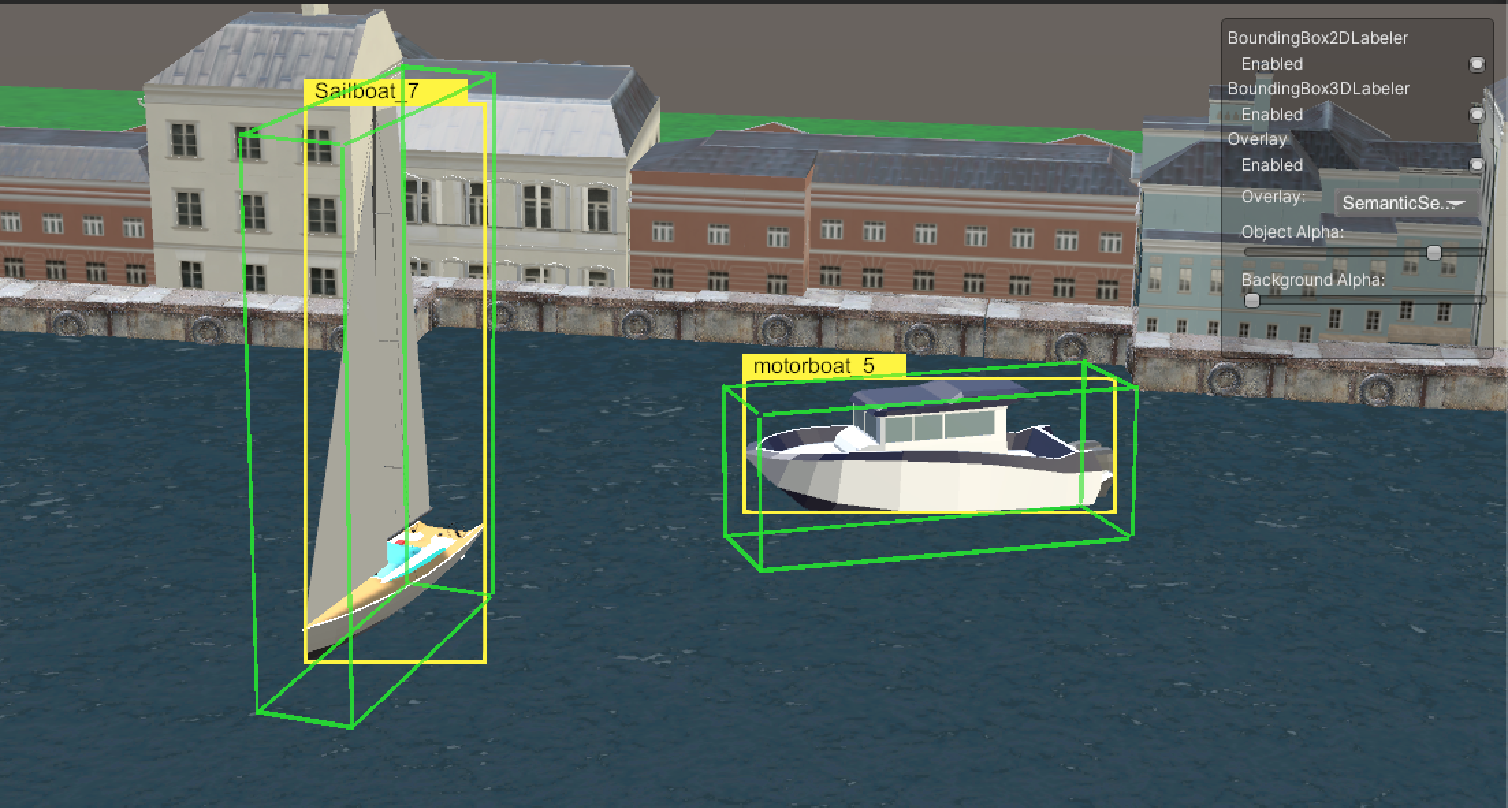
\includegraphics[width=0.7\textwidth]{Figures/boundingbox.png}
    \caption{Illustration of bounding boxes, with rectangular regions used to localize objects.}
    \label{fig:image2}
\end{figure}

\begin{figure}[H]
    \centering
    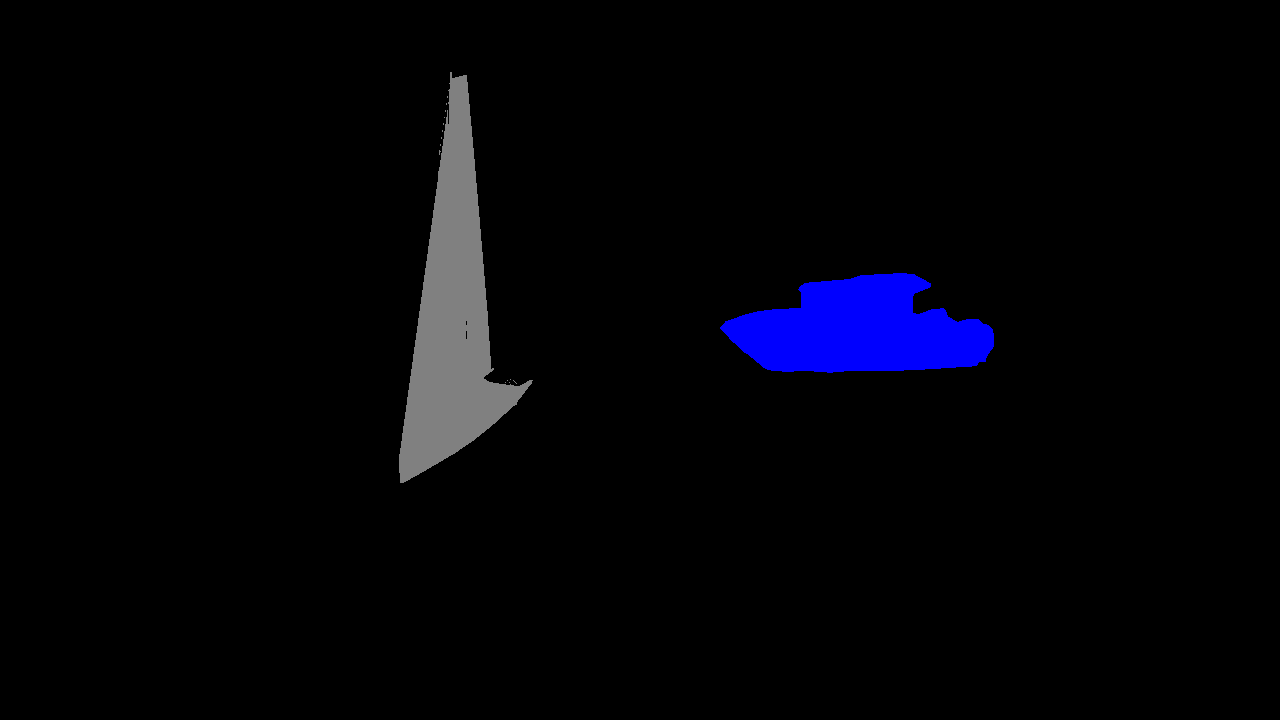
\includegraphics[width=0.7\textwidth]{Figures/segmentation_2.png}
    \caption{Visualization of segmentation, which divide the image into precise pixel-level regions.}
    \label{fig:image3}
\end{figure}



\subsection{Advantages with Synthetic Labeling}
Labeling in synthetic images is a big advantage compare to real images. Using real images requires manual effort for labeling, which involves identifying and annotating each object in the dataset. As dataset sizes grows, manual labeling becomes impractical. Annotating thousands of real-world images needs a lot of human labor and can include inconsistencies, potentially impacting the model accuracy \cite{nikolenko2021synthetic}.\\

\noindent In contrast, synthetic images provide the advantage of automatic labeling during the generation process. Platforms like Unity offer automated labeling capabilities via the Perception Package \cite{unity-perception2022}. This ensures pixel-perfect annotations, including bounding boxes and segmentation masks with no manual intervention. The automated process delivers consistent, high-quality annotations for every image while saving time and effort.


\section{Balancing Realism in Synthetic Data}
While synthetic image generation offers numerous benefits for computer vision models, a key challenge is achieving sufficient realism. The domain gap between synthetic and real-world data can significantly impact model performance \cite{nikolenko2021synthetic}.  Although it is possible to create highly realistic scenes, some aspects remain particularly difficult to simulate. For instance, dynamic surfaces like water in maritime applications can be a challenge due to its complex behavior with reflections and refractions \cite{waterrendering}. Similarly, obtaining realistic 3D renderings of objects like boats and other maritime structures can be difficult.\\

\noindent Going for a realistic synthetic datasets can be expensive and time consuming and may outweigh the benefits. Instead, specific optimizations and techniques can help bridge the gap between synthetic and real-world data \cite{nikolenko2021synthetic, jimaging8110310}. By balancing realism and practicality, synthetic datasets can achieve a level that meets the needs of specific applications without excessive computational costs.


\section{The Future of Synthetic Images}
\label{gan}
Using AI to generate images for computer vision models has become an increasingly powerful tool, with Generative Adversarial Networks (GANs) being popular in this field. GANs consist of two neural networks that work in a competitive process to create realistic synthetic data. The generator produces fake data, while the discriminator evaluates whether the data is real or fake, with both networks improving through this competition. This dynamic has made GANs highly effective for tasks like image generation, domain adaptation and creating privacy-preserving synthetic datasets. Despite their potential, training GANs can be challenging due to the risk of producing data with limited diversity. These challenges can limit the models ability to generalize and innovate \cite{gan}. GANs and other AI-driven innovations are helping reduce the time and cost of creating datasets, while also enabling the simulation of complex scenarios and environments. However, using AI to train AI introduces additional risks such as overfitting and hallucination. This is when models generate outputs that are not only inaccurate but may also be entirely fictional or irrelevant \cite{hallucination}. Hallucinations often arise from poor-quality training data that the model may overfit during training, leading to bad results. Tackling this challenge requires the development of new techniques to detect and correct these errors, ensuring more reliable synthetic data.
